\documentclass[mathserif,xcolor=dvipsnames,hyperref={bookmarks=true}]{beamer}
%\documentclass[mathserif,xcolor=dvipsnames,handout]{beamer}
\usepackage[scaled]{helvet}
\usepackage{eulervm}
\usepackage{courier}
\usepackage{listings}
%\usepackage{xmpincl}  % http://www.ctan.org/tex-archive/macros/latex/contrib/xmpincl/
%\includexmp{byncsa}
%\usepackage[binary,amssymb]{SIunits}
\usefonttheme{structurebold}
\usecolortheme[named=Maroon]{structure}
\usetheme{Antibes}
\usecolortheme{lily}
\useoutertheme{infolines}
\setbeamertemplate{navigation symbols}{}
\usepackage{xmpmulti} % for \multiinclude

\newcommand{\mytitle}{Making Creative Commons More Useful by Applying Usage Management}
\newcommand{\myshorttitle}{CC More Useful with Usage Management}
\newcommand{\myauthor}{Matthew Paul Bohnsack}
\newcommand{\myshortauthor}{Matthew Bohnsack}

% We should look for graphics in these directories
\graphicspath{
{resources/logos/UNM/}
{../resources/usecases/usecase1/}
{../resources/usecases/usecase2/}
{../resources/component-design/}
{../resources/implementation/}
{../resources/flickr/}
{../resources/cc/}
{../resources/RDF/}
{../resources/pdfviewer/}
}

% Settings for code/text listings
\lstset{ %
basicstyle=\tiny\ttfamily,       % the size of the fonts that are used for the code and the font
%numbers=left,                   % where to put the line-numbers
%numberstyle=\footnotesize,      % the size of the fonts that are used for the line-numbers
%stepnumber=2,                   % the step between two line-numbers. If it's 1, each line 
                                 % will be numbered
%numbersep=5pt,                  % how far the line-numbers are from the code
%backgroundcolor=\color{white},  % choose the background color. You must add \usepackage{color}
showspaces=false,               % show spaces adding particular underscores
showstringspaces=false,         % underline spaces within strings
showtabs=false,                 % show tabs within strings adding particular underscores
frame=shadowbox,                   % adds a frame around the code
rulesepcolor=\color{Gray},
tabsize=2,                      % sets default tabsize to 2 spaces
%captionpos=b,                   % sets the caption-position to bottom
breaklines=true,                % sets automatic line breaking
breakatwhitespace=false,        % sets if automatic breaks should only happen at whitespace
%title=\lstname,                 % show the filename of files included with \lstinputlisting;
%                                % also try caption instead of title
%escapeinside={\%*}{*)},         % if you want to add a comment within your code
%morekeywords={*,...}            % if you want to add more keywords to the set
}

% Check this for automating the creation of different files: slides, handouts, etc...
% http://www.pletscher.org/writings/latex/Makefile
% http://www.pletscher.org/writings/latex/beamer.php

% Do this if handouts...
%\usepackage{pgfpages}
%\pgfpagesuselayout{2 on 1}[letterpapper,border shrink=5mm]
%\mode<handout>{\setbeamercolor{background canvas}{bg=black!5}}

\usepackage{default}

\title[\myshorttitle]{\mytitle}
%\subtitle{Including a Usage Management Example in Ruby}
\author[\myshortauthor]{\myauthor}
\institute[UNM]{University of New Mexico\\Albuquerque, New Mexico USA\\[2ex]\texttt{bohnsack@gmail.com}}
%\date{Friday March 25, 2011}

\newcommand{\putat}[3]{\begin{picture}(0,0)(0,0)\put(#1,#2){#3}\end{picture}}

%\lstset{language=bash,rulesepcolor=\color{Gray},frame=shadowbox,basicstyle=\tiny\ttfamily}

\begin{document}

\AtBeginSection[]
{
\begin{frame}{Table of Contents}
\tableofcontents[currentsection,hideothersubsections]
\end{frame}
}

% make covered bullet points sill show up, but muted
\setbeamercovered{transparent=7}


%%%%%%%%%%%%%%%%%%%%%%%%%%%%%%%%%%%%%%%%%%%%%%%%%%%%%%%%%%%%%%%%%%%%%
% Title
%%%%%%%%%%%%%%%%%%%%%%%%%%%%%%%%%%%%%%%%%%%%%%%%%%%%%%%%%%%%%%%%%%%%%
\begin{frame}
    \titlepage
    \begin{center}
        
\includegraphics[width=0.24\textwidth]{UNM_logo_PMS200C.pdf}
    \end{center}
\end{frame}

%%%%%%%%%%%%%%%%%%%%%%%%%%%%%%%%%%%%%%%%%%%%%%%%%%%%%%%%%%%%%%%%%%%%%
\section{Introduction}
%%%%%%%%%%%%%%%%%%%%%%%%%%%%%%%%%%%%%%%%%%%%%%%%%%%%%%%%%%%%%%%%%%%%%

    \subsection{Abstract}
    %%%%%%%%%%%%%%%%%%%%%%%%%%%%%%%%%%%%%%%%%%%%%%%%%%%%%%%%%%%%%%%%%%%%%
    \begin{frame}[t]
        \frametitle{Abstract}
    \end{frame}

    \subsection{Motivation}
    %%%%%%%%%%%%%%%%%%%%%%%%%%%%%%%%%%%%%%%%%%%%%%%%%%%%%%%%%%%%%%%%%%%%%
    \begin{frame}[t]
        \frametitle{Motivation}
        \begin{itemize}
            \item<2-> Creative Commons is being used more and more
            \item<3-> Easy to find images on the web licensed under different CC licenses
            \item<4-> Very easy to make a mash-up document containing ``found images''
            \item<5-> Not so easy to make sure you're following all the rules when
                  you create derivative works (mash-ups)
            \item<6-> Is your intended use 100\% compliant with dozens or hundreds
                  of assets you're using, each of which might have a slightly different
                  Creative Commons license?
            \item<7-> If an asset you want to use has a license incompatible with
                  your intended use, is there an easy way for you to acquire an alternative
                  license that lets you use the asset in the way you want to?
            \item<8-> Doing this sort of thing today is pretty difficult
            \item<9-> Adding some automated machine reasoning to the process could
                  make it all much easier and possibly make the proper use of combined CC content
                  a more widespread practice
        \end{itemize}
    \end{frame}

    \subsection{Creative Commons}
    %%%%%%%%%%%%%%%%%%%%%%%%%%%%%%%%%%%%%%%%%%%%%%%%%%%%%%%%%%%%%%%%%%%%%

    \begin{frame}[t]
        \frametitle{Creative Commons Overview}
        \begin{itemize}
            \item<2-> Creative commons is a nonprofit organization that works to
                  increase the amount of creativity available in ``the commons''
            \item<3-> Provides free, easy-to-use legal tools that provide a simple,
                  standardized way to pre-clear usage rights to creative work for
                  copyright owners
            \item<4-> Lets copyright holders easily change from default of ``all
                  rights reserved'' to ``some rights reserved''
            \item<5-> Not an alternative to copyright
            \item<6-> Applies on top of copyright
            \item<7-> Guidelines for marking text, images, audio, and video
            \item<8-> Guidelines for publishing via a file sharing network or
                  social networking site
            \item<9-> Some support for embedding license information as meta-data
                  within digital files
        \end{itemize}
    \end{frame}

    \begin{frame}[t]
        \frametitle{Creative Commons Overview (cont.)}
        \begin{itemize}
            \item<2-> Not changeable or revocable
            \item<3-> I.e., once someone has received a copy, the work is
                  perpetually licensed under the license it was received under
            \item<4-> View is always permissible under CC
            \item<5-> Non-exclusive licenses possible
        \end{itemize}
    \end{frame}

    \begin{frame}[t]
        \frametitle{CC Licenses Have Three Layers}
            \begin{itemize}
                \item<2-> Machine Readable (CC Rights Expression Language - CC REL)
                \item<3-> Human Readable (Commons Deed)
                \item<4-> Legal Code (Lawyer Readable)
            \end{itemize}
        \begin{center}
          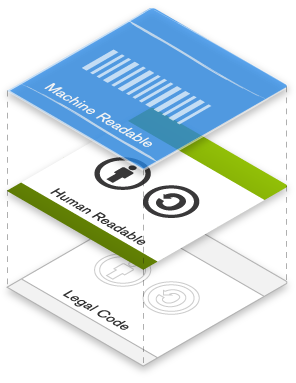
\includegraphics[width=0.4\textwidth]{license_layers.png}
        \end{center}
    \end{frame}

     \begin{frame}[t]
         \frametitle{Creative Commons Licenses}
         \begin{itemize}
             \item<2-> Six licenses are provided by CC, not including the
             complications of locale-specific licenses, license versions, or
             CC0 (Public Domain ``no rights reserved'')
             \begin{enumerate}
               \item<3-> 
\includegraphics[width=0.1\textwidth]{by.pdf}\ Attribution
               / CC BY
               \item<4-> 
\includegraphics[width=0.1\textwidth]{by_sa.pdf}\
               Attribution-ShareAlike / CC BY-SA
               \item<5-> 
\includegraphics[width=0.1\textwidth]{by_nd.pdf}\
               Attribution-NoDerivs / CC BY-ND
               \item<6-> 
\includegraphics[width=0.1\textwidth]{by_nc.pdf}\
               Attribution-NonCommercial / CC BY-NC
               \item<7-> 
\includegraphics[width=0.1\textwidth]{by_nc_sa.pdf}\
               Attribution-NonCommercial-ShareAlike / CC BY-NC-SA
               \item<8-> 
\includegraphics[width=0.1\textwidth]{by_nc_nd.pdf}\
               Attribution-NonCommercial-NoDerivs / CC BY-NC-ND
             \end{enumerate}
             \item<9-> Non-exclusive licenses, yielding CC+:
             \texttt{http://wiki.creativecommons.org/CCPlus} \\
               
\includegraphics[width=0.1\textwidth]{by_nc_sa.pdf}
               +
\includegraphics[width=0.1\textwidth]{CommercialLicenseButton.pdf}
         \end{itemize}
     \end{frame}
     % https://creativecommons.org/about/downloads

    % 1 %%%%%%%%%%%%%%%%%%%%%%%%%%%%%%%%%%%%%%%%%%%%%%%%%%%%%%%%%%%%%%%%%%%%
    \begin{frame}[t]
        \frametitle{Attribution}
        
\includegraphics[width=0.1\textwidth]{by.pdf}\  This license lets
        others distribute, remix, tweak, and build upon your work, even
        commercially, as long as they credit you for the original creation.
        This is the most accommodating of the licenses offered.  Recommended
        for maximum dissemination and use of licensed materials.
        \vspace{0.1in}
        \begin{itemize}
            \item You are free:
            \begin{itemize}
                \item 
\includegraphics[width=0.03\textwidth]{share.pdf}\
                \textbf{to Share} -- to copy, distribute, and transmit the work
                \item 
\includegraphics[width=0.03\textwidth]{remix.pdf}\
                \textbf{to Remix} -- to adapt the work
            \end{itemize}
            \item Under the following conditions:
            \begin{itemize}
                \item 
\includegraphics[width=0.03\textwidth]{bigby.pdf}\
                \textbf{Attribution} -- You must attribute the work in the
                manner specified by the author or licensor (but not in any way
                that suggests that they endorse you or your use of the work).
            \end{itemize}
        \end{itemize}
    \end{frame}

    % 2 %%%%%%%%%%%%%%%%%%%%%%%%%%%%%%%%%%%%%%%%%%%%%%%%%%%%%%%%%%%%%%%%%%%%
    \begin{frame}[t]
        \frametitle{Attribution-ShareAlike}
        
\includegraphics[width=0.1\textwidth]{by_sa.pdf}\ This
        license lets others remix, tweak, and build upon your work even for
        commercial purposes, as long as they credit you and license their new
        creations under the identical terms. This license is often compared to
        free and open source software licenses. All new works based on yours
        will carry the same license, so any derivatives will also allow
        commercial use.
        \vspace{0.1in}
        \begin{itemize}
            \item You are free:
            \begin{itemize}
                \item 
\includegraphics[width=0.03\textwidth]{share.pdf}\
                \textbf{to Share} -- to copy, distribute, and transmit the work
                \item 
\includegraphics[width=0.03\textwidth]{remix.pdf}\
                \textbf{to Remix} -- to adapt the work
            \end{itemize}
            \item Under the following conditions:
            \begin{itemize}
                \item 
\includegraphics[width=0.03\textwidth]{bigby.pdf}\
                \textbf{Attribution} -- You must attribute the work in the
                manner specified by the author or licensor (but not in any way
                that suggests that they endorse you or your use of the work).
                \item 
\includegraphics[width=0.03\textwidth]{sa.pdf}\
                \textbf{Share Alike} -- If you alter, transform, or build upon
                this work, you may distribute the resulting work only under the
                same or similar license to this one.
            \end{itemize}
        \end{itemize}
    \end{frame}

    % 3 %%%%%%%%%%%%%%%%%%%%%%%%%%%%%%%%%%%%%%%%%%%%%%%%%%%%%%%%%%%%%%%%%%%%
    \begin{frame}[t]
        \frametitle{Attribution-NoDerivs}
        
\includegraphics[width=0.1\textwidth]{by_nd.pdf}\ This
        license allows for redistribution, commercial and non-commercial, as long as it
        is passed along unchanged and in whole, with credit to you.
        \vspace{0.1in}
        \begin{itemize}
            \item You are free:
            \begin{itemize}
                \item 
\includegraphics[width=0.03\textwidth]{share.pdf}\
                \textbf{to Share} -- to copy, distribute, and transmit the work
            \end{itemize}
            \item Under the following conditions:
            \begin{itemize}
                \item 
\includegraphics[width=0.03\textwidth]{bigby.pdf}\
                \textbf{Attribution} -- You must attribute the work in the
                manner specified by the author or licensor (but not in any way
                that suggests that they endorse you or your use of the work).
                \item 
\includegraphics[width=0.03\textwidth]{nd.pdf}\
                \textbf{No Derivative Works} -- You may not alter, transform,
                or build upon this work.
            \end{itemize}
        \end{itemize}
    \end{frame}

    % 4 %%%%%%%%%%%%%%%%%%%%%%%%%%%%%%%%%%%%%%%%%%%%%%%%%%%%%%%%%%%%%%%%%%%%
    \begin{frame}[t]
        \frametitle{Attribution-NonCommercial}
        
\includegraphics[width=0.1\textwidth]{by_nc.pdf}\ This license lets
        others remix, tweak, and build upon your work non-commercially, and
        although their new works must also acknowledge you and be
        non-commercial, they don't have to license their derivative works on
        the same terms.
        \vspace{0.1in}
        \begin{itemize}
            \item You are free:
            \begin{itemize}
                \item 
\includegraphics[width=0.03\textwidth]{share.pdf}\
                \textbf{to Share} -- to copy, distribute, and transmit the work
                \item 
\includegraphics[width=0.03\textwidth]{remix.pdf}\
                \textbf{to Remix} -- to adapt the work
            \end{itemize}
            \item Under the following conditions:
            \begin{itemize}
                \item
                
\includegraphics[width=0.03\textwidth]{bigby.pdf}\
                \textbf{Attribution} -- You must attribute the work in the
                manner specified by the author or licensor (but not in any way
                that suggests that they endorse you or your use of the work).
                \item 
\includegraphics[width=0.03\textwidth]{nc.pdf}\
                \textbf{Noncommercial} -- You may not use this work for
                commercial purposes.
            \end{itemize}
        \end{itemize}
    \end{frame}

    % 5 %%%%%%%%%%%%%%%%%%%%%%%%%%%%%%%%%%%%%%%%%%%%%%%%%%%%%%%%%%%%%%%%%%%%
    \begin{frame}[t]
        \frametitle{Attribution-NonCommercial-ShareAlike}
        
\includegraphics[width=0.1\textwidth]{by_nc_sa.pdf}\ This license lets
        others remix, tweak, and build upon your work non-commercially, as long
        as they credit you and license their new creations under the identical
        terms.
        \vspace{0.1in}
        \begin{itemize}
            \item You are free:
            \begin{itemize}
                \item 
\includegraphics[width=0.03\textwidth]{share.pdf}\
                \textbf{to Share} -- to copy, distribute, and transmit the work
                \item 
\includegraphics[width=0.03\textwidth]{remix.pdf}\
                \textbf{to Remix} -- to adapt the work
            \end{itemize}
            \item Under the following conditions:
            \begin{itemize}
                \item 
\includegraphics[width=0.03\textwidth]{bigby.pdf}\
                \textbf{Attribution} -- You must attribute the work in the
                manner specified by the author or licensor (but not in any way
                that suggests that they endorse you or your use of the work).
                \item 
\includegraphics[width=0.03\textwidth]{nc.pdf}\
                \textbf{Noncommercial} -- You may not use this work for
                commercial purposes.
                \item 
\includegraphics[width=0.03\textwidth]{sa.pdf}\
                \textbf{Share Alike} -- If you alter, transform, or build upon
                this work, you may distribute the resulting work only under the
                same or similar license to this one.
            \end{itemize}
        \end{itemize}
    \end{frame}

    % 6 %%%%%%%%%%%%%%%%%%%%%%%%%%%%%%%%%%%%%%%%%%%%%%%%%%%%%%%%%%%%%%%%%%%%
    \begin{frame}[t]
        \frametitle{Attribution-NonCommercial-NoDerivs}
        
\includegraphics[width=0.1\textwidth]{by_nc_nd.pdf}\ This license is
        the most restrictive of the six main licenses, only allowing others to
        download your works and share them with others as long as they credit
        you, but they can't change them in any way or use them commercially.
        \vspace{0.1in}
        \begin{itemize}
            \item You are free:
            \begin{itemize}
                \item 
\includegraphics[width=0.03\textwidth]{share.pdf}\
                \textbf{to Share} -- to copy, distribute, and transmit the work
            \end{itemize}
            \item Under the following conditions:
            \begin{itemize}
                \item 
\includegraphics[width=0.03\textwidth]{bigby.pdf}\
                \textbf{Attribution} -- You must attribute the work in the
                manner specified by the author or licensor (but not in any way
                that suggests that they endorse you or your use of the work).
                \item 
\includegraphics[width=0.03\textwidth]{nc.pdf}\
                \textbf{Noncommercial} -- You may not use this work for
                commercial purposes.
                \item 
\includegraphics[width=0.03\textwidth]{nd.pdf}\
                \textbf{No Derivative Works} -- You may not alter, transform,
                or build upon this work.
            \end{itemize}
        \end{itemize}
    \end{frame}

    \begin{frame}[t]
        \frametitle{CC REL}
        \begin{itemize}
            \item The Creative Commons Rights Expression Language
            \item RDFa (Resource Description Framework in attributes) for HTML
            Web pages and resources referenced therein
            \item XMP (Extensible Metadata Platform) for stand-alone media
            \item \texttt{http://wiki.creativecommons.org/CC\_REL}
        \end{itemize}
    \end{frame}

\begin{frame}[fragile]
\frametitle{RDFa in HTML}
        \begin{itemize}
            \item Can simply associate web content with a CC license:
        \end{itemize}
\lstinputlisting[language=HTML]{../listings/RDFaExample.html}
        \begin{itemize}
            \item But what are the semantics of \url{http://creativecommons.org/licenses/by/3.0/}?
        \end{itemize}
\end{frame}

\begin{frame}[t]
\frametitle{License Deed Webpage}
        \begin{itemize}
            %\item Looking at license URL as rendered
            %in browser, it's not obvious how a machine could
            %derive semantics:
            \item Can a machine derive this page's semantics?
        \end{itemize}
        \begin{center}
            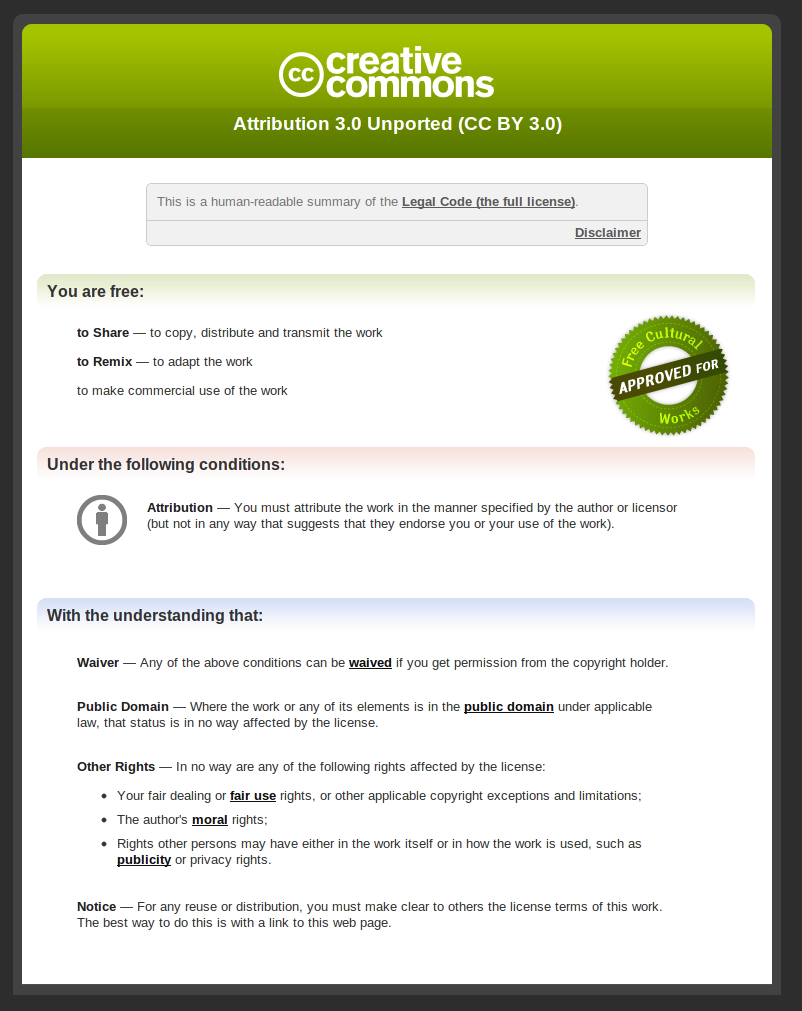
\includegraphics[height=0.8\textheight]{cc-deed-rendered-in-browser.png}
        \end{center}
\end{frame}

\begin{frame}[fragile]
\frametitle{RDF Embedded in License Deed Webpage}
        \begin{itemize}
            \item The previous webpage contains the following embedded RDF:
        \end{itemize}
\lstinputlisting[language=HTML]{../listings/CC-deed-embeded-RDF.xml}
        \begin{itemize}
            \item From this, a machine can determine that this license:
            \begin{itemize}
                \item Permits:
                    \begin{itemize}
                        \item \texttt{\#DerivativeWorks}, \texttt{\#Distribution}, \texttt{\#Reproduction}
                    \end{itemize}
                \item Requires:
                    \begin{itemize}
                        \item \texttt{\#Attribution}, \texttt{\#Notice}
                    \end{itemize}
            \end{itemize}
            \item However, what do these things mean?  How are they implemented?
        \end{itemize}
\end{frame}

\begin{frame}[t]
\frametitle{RDFa Embedded in License Deed Webpage}
        \begin{itemize}
            \item In addition to the RDF shown on previous slide, CC License Deeds also have embedded RDFa
            \item You can see that a machine can parse this data with something
            like the RDFa Distiller and Parser Tool:
        \end{itemize}
        \begin{center}
            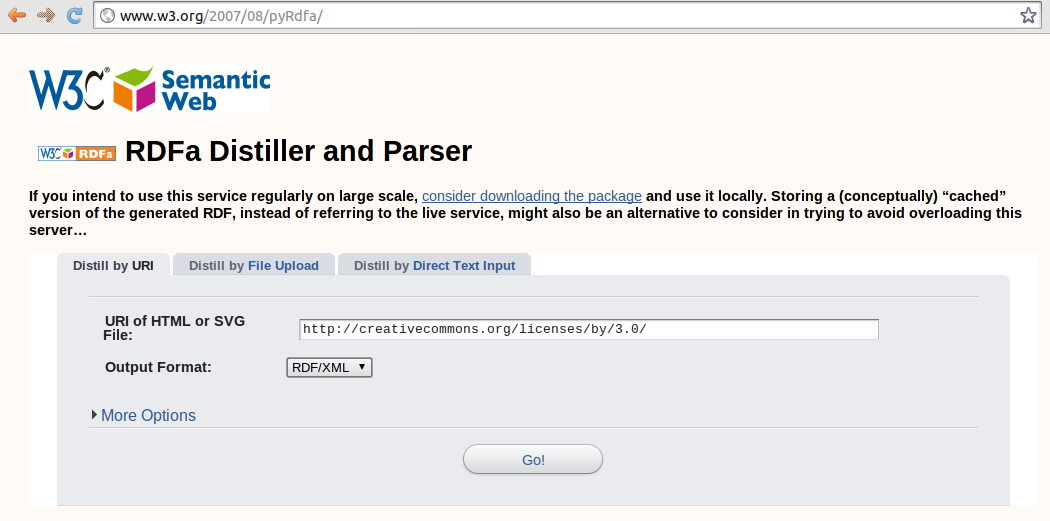
\includegraphics[width=0.8\textwidth]{RDFa-distiller.png}
        \end{center}
\end{frame}


\begin{frame}[fragile]
\frametitle{RDF Generated by RDFa Distiller}
\lstinputlisting[language=HTML]{../listings/RDF-from-RDFa-distiller.xml}
\end{frame}

\begin{frame}[t]
\frametitle{CC RDF Schema}
        \begin{itemize}
            \item License RDF(a) references \texttt{\#DerivativeWorks}, etc., in the CC namespace that's defined by a schema that's human-readable and machine-readable RDF.
            \item But... how immediately machine actionable is this schema?
            \item Partial screenshot below:
        \end{itemize}
        \begin{center}
            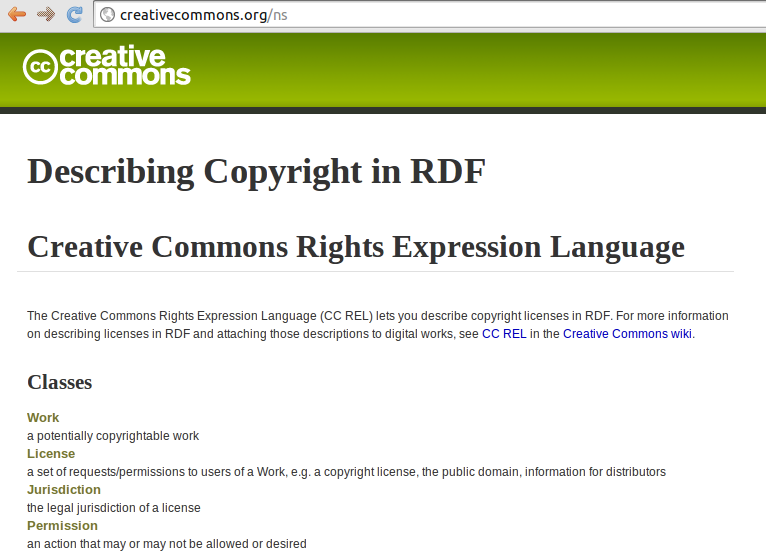
\includegraphics[width=0.4\textwidth]{schema-screenshot-partial.png}
        \end{center}
        \begin{itemize}
            \item We would like to investigate replacing or augmenting RDF(a)
            in the license deed with a license that's described with our DSL
        \end{itemize}
\end{frame}

\begin{frame}[t]
\frametitle{DSL-Based License Deed}
    \begin{itemize}
        \item By investigating replacing the contents of a license like
        \url{http://creativecommons.org/licenses/by/3.0/} with something that
        expresses the license in terms our DSL, we hope to:
        \begin{itemize}
            \item Maintain equivalent license semantics
            \item Express the semantics in a form that is easier for humans to read and write
            \item Enable a machine to more directly execute the license and reason over it
        \end{itemize}
    \end{itemize}
\end{frame}

    \begin{frame}[t]
        \frametitle{XMP for Stand-Alone Media}
        \begin{itemize}
            \item \LaTeX\ package on CTAN (\texttt{xmpincl})
        \end{itemize}
        \begin{center}
            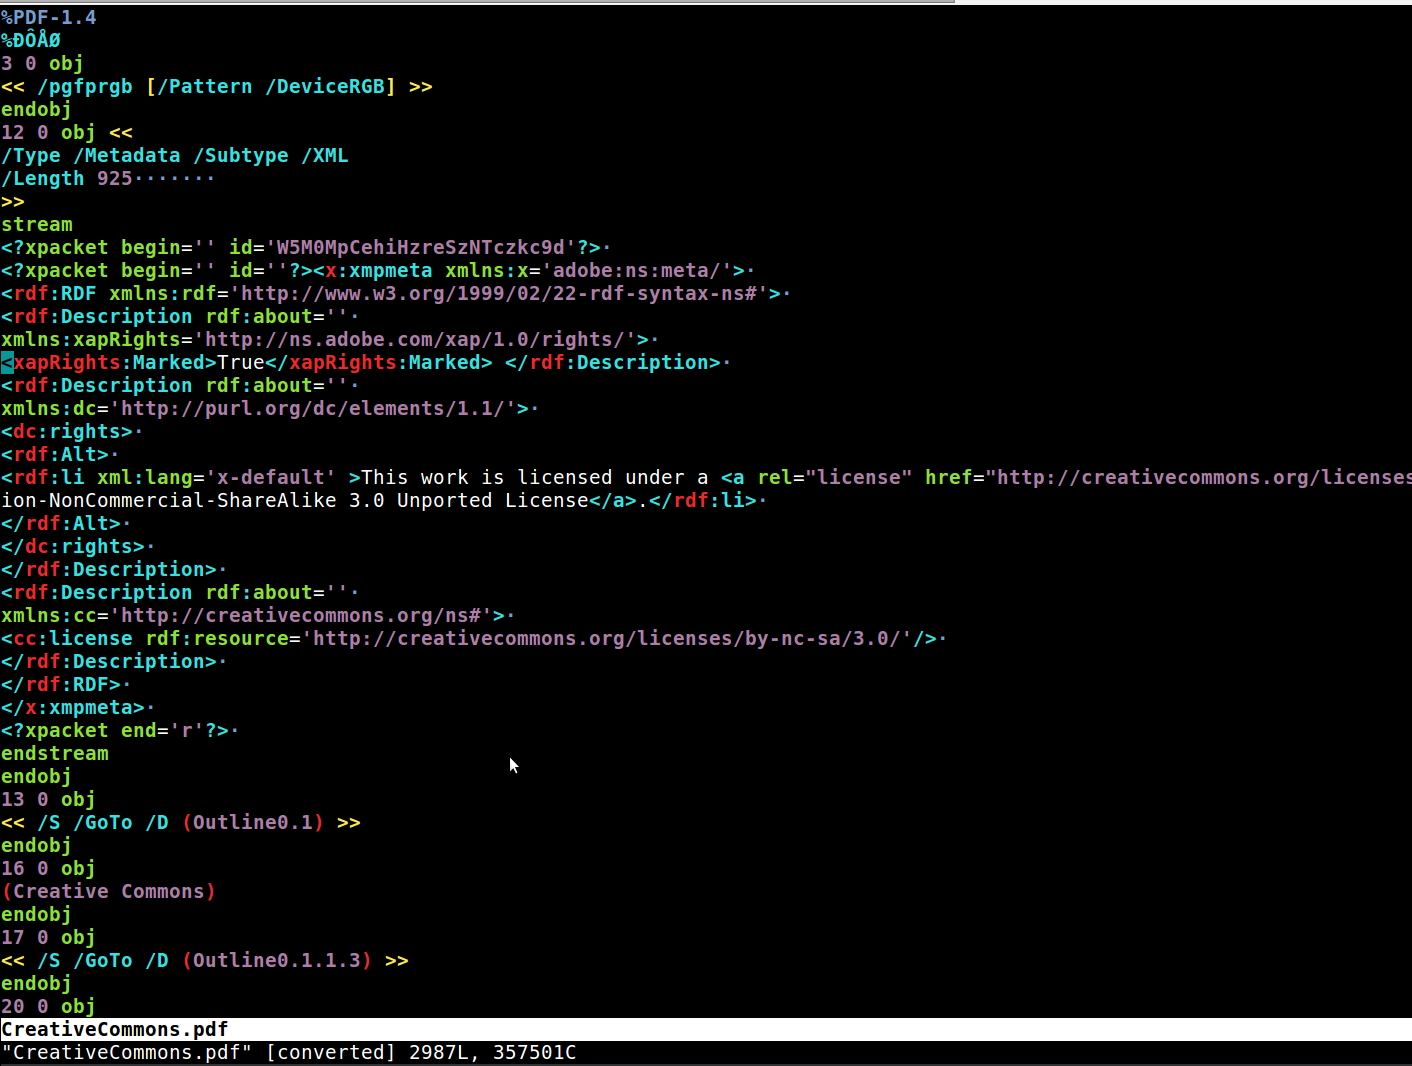
\includegraphics[width=0.7\textwidth]{embedded_xmp.png}
        \end{center}
    \end{frame}

    \subsection{Flickr}
    %%%%%%%%%%%%%%%%%%%%%%%%%%%%%%%%%%%%%%%%%%%%%%%%%%%%%%%%%%%%%%%%%%%%%
    \begin{frame}[t]
        \frametitle{Flickr 1}
        \begin{center}
            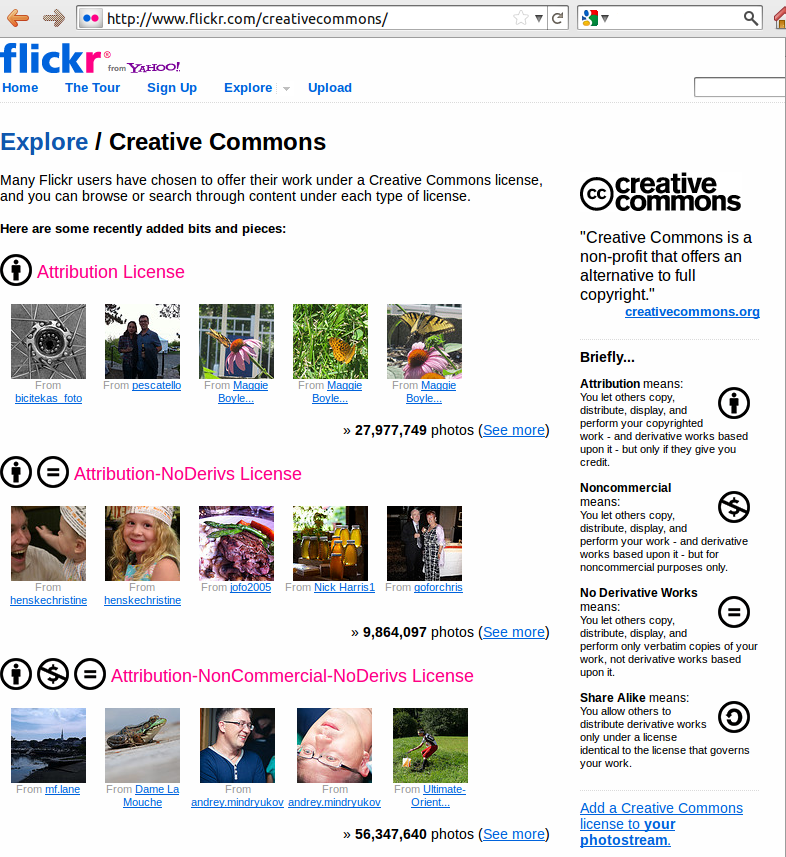
\includegraphics[height=0.8\textheight]{explore-cc-photos-on-flickr.png}
        \end{center}
    \end{frame}
    \begin{frame}[t]
        \frametitle{Flickr 2}
        \begin{center}
            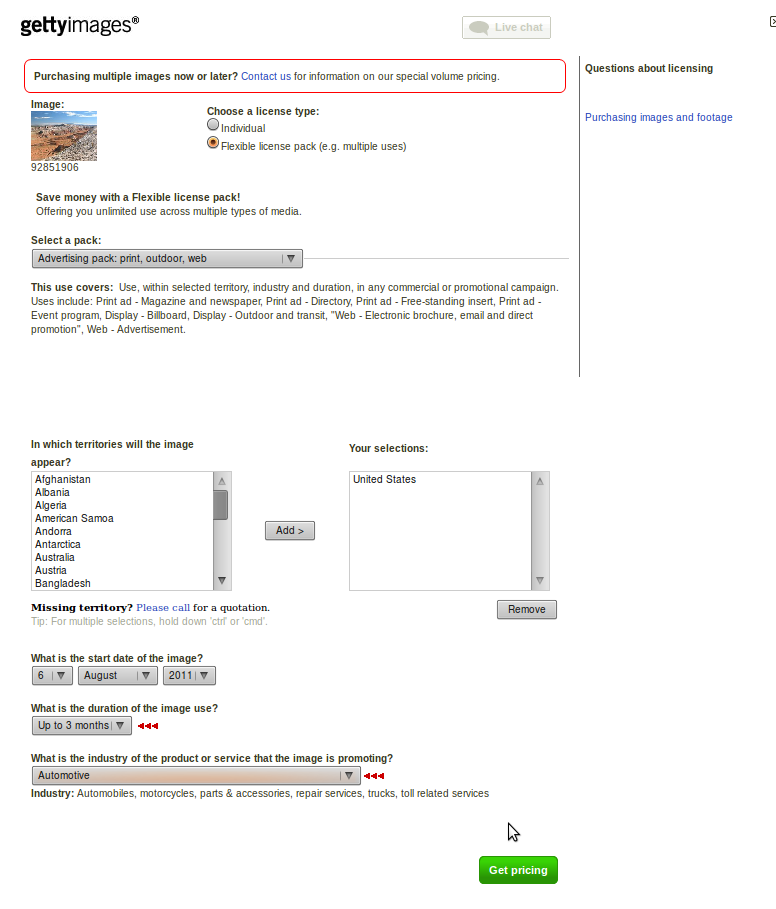
\includegraphics[height=0.8\textheight]{gettyimages-pricing.png}
        \end{center}
    \end{frame}
    \begin{frame}[t]
        \frametitle{Flickr 3}
        \begin{center}
            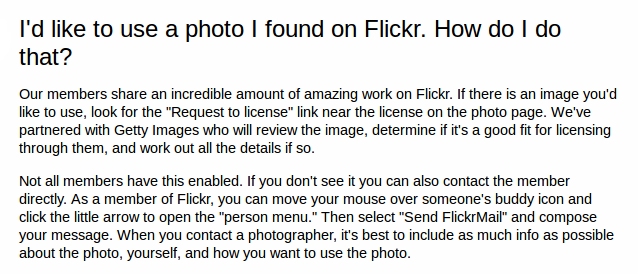
\includegraphics[width=0.8\textwidth]{i-would-like-to-use-a-photo-i-found-on-flickr.png}
        \end{center}
    \end{frame}
    \begin{frame}[t]
        \frametitle{Flickr 4}
        \begin{center}
            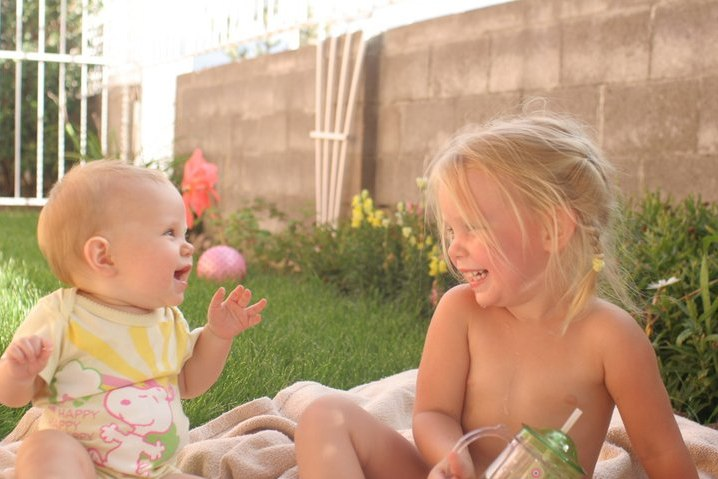
\includegraphics[width=0.8\textwidth]{katherine-and-evelyn.jpg}
        \end{center}
    \end{frame}
    \begin{frame}[t]
        \frametitle{Flickr 5}
        \begin{center}
            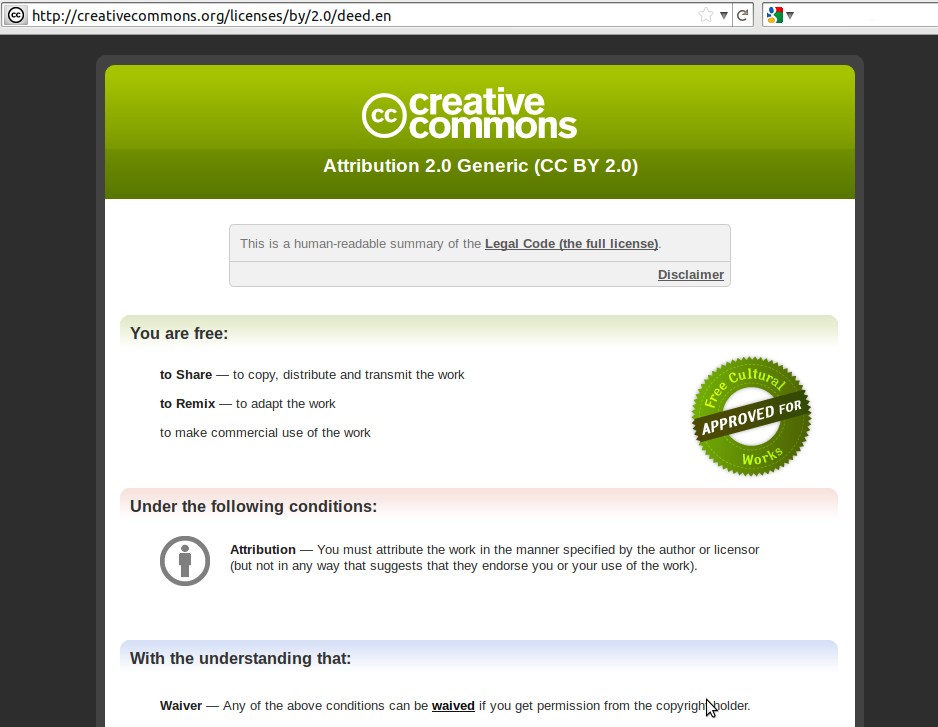
\includegraphics[height=0.8\textheight]{link-to-cc-license-from-flickr.png}
        \end{center}
    \end{frame}
    \begin{frame}[t]
        \frametitle{Flickr 6}
        \begin{center}
            
\includegraphics[width=0.8\textwidth]{request-to-license1.png}
        \end{center}
    \end{frame}
    \begin{frame}[t]
        \frametitle{Flickr 7}
        \begin{center}
            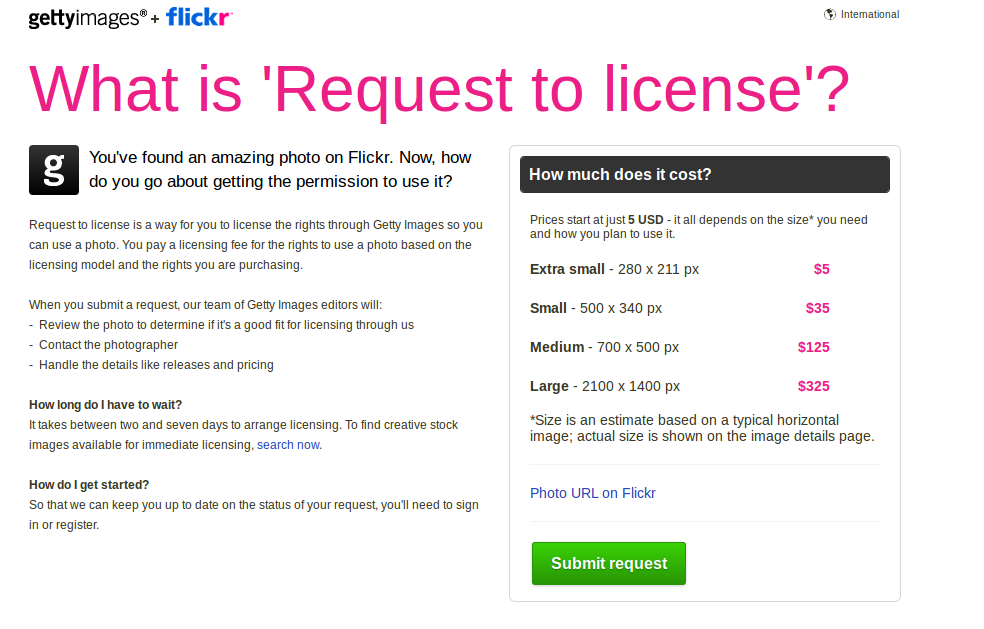
\includegraphics[height=0.8\textheight]{request-to-license2.png}
        \end{center}
    \end{frame}
    \begin{frame}[t]
        \frametitle{Flickr 8}
        \begin{center}
            \includegraphics[height=0.8\textheight]{select-cc-license-for-your-photo-on-flickr.png}
        \end{center}
    \end{frame}
    \begin{frame}[t]
        \frametitle{Flickr 9}
        \begin{center}
            \includegraphics[height=0.8\textheight]{set-you-license-on-flickr.png}
        \end{center}
    \end{frame}
    \begin{frame}[t]
        \frametitle{Flickr 10}
        \begin{center}
            \includegraphics[width=0.8\textwidth]{view-cc-licensed-photo-on-flickr.png}
        \end{center}
    \end{frame}
    \begin{frame}[t]
        \frametitle{Flickr 11}
        \begin{center}
            \includegraphics[height=0.8\textheight]{view-photo-and-see-cc-license.png}
        \end{center}
    \end{frame}
    \begin{frame}[t]
        \frametitle{Flickr 12}
        \begin{center}
            \includegraphics[height=0.8\textheight]{view-your-own-photo-on-flickr.png}
        \end{center}
    \end{frame}
    \begin{frame}[t]
        \frametitle{Flickr 13}
        \begin{center}
            \includegraphics[width=0.8\textwidth]{want-to-license-your-photos-through-getty-images.png}
        \end{center}
    \end{frame}
    \begin{frame}[t]
        \frametitle{Flickr 14}
        \begin{center}
            \includegraphics[width=0.8\textwidth]{want-to-license-your-photos-through-getty-images2.png}
        \end{center}
    \end{frame}


%xmp-meta-data-in-eog.png
%[mpbohns@saskatchewan ~/rcs/Matthew_Bohnsack_MS_Thesis/resources]$ ls -1 pdfviewer/
%evince-showing-license-embedded-with-xmpincl.png

    \subsection{Usage Management}
    %%%%%%%%%%%%%%%%%%%%%%%%%%%%%%%%%%%%%%%%%%%%%%%%%%%%%%%%%%%%%%%%%%%%%
    \begin{frame}[t]
        \frametitle{Usage Management}
        \begin{itemize}
            \item<2-> AAA aAAAA aaaaa AAAAAAAAAA
            \item<3-> Bb bb b b BBBBBBBBBB bbbBB
            \item<4-> c CCCC ccCCC ccc cCCCcCc C
        \end{itemize}
    \end{frame}

%%%%%%%%%%%%%%%%%%%%%%%%%%%%%%%%%%%%%%%%%%%%%%%%%%%%%%%%%%%%%%%%%%%%%
\section{System Design}
%%%%%%%%%%%%%%%%%%%%%%%%%%%%%%%%%%%%%%%%%%%%%%%%%%%%%%%%%%%%%%%%%%%%%

    \subsection{Use Cases}
    %%%%%%%%%%%%%%%%%%%%%%%%%%%%%%%%%%%%%%%%%%%%%%%%%%%%%%%%%%%%%%%%%%%%%

    % Use Case #1 %%%%%%%%%%%%%%%%%%%%%%%%%
    \begin{frame}[t]
        \setbeamercovered{invisible}
        \frametitle{Use Case \#1: Simple Use}
        \begin{center}
            % The "[<+>]" thing means totally replace the prior graphic each
            % time.  Otherwise the default behavior is to stack all graphics
            % on top of each other.
            \multiinclude[<+>][format=pdf,graphics={width=0.51\textwidth}]{usecase1}
        \end{center}
    \end{frame}

    % Use Case #2 %%%%%%%%%%%%%%%%%%%%%%%%%
    \begin{frame}[t]
        \setbeamercovered{invisible}
        \frametitle{Use Case \#2: Including the CC+ Broker Service}
        \begin{center}
            \multiinclude[<+>][format=pdf,graphics={width=0.9\textheight}]{usecase2}
        \end{center}
    \end{frame}

    \subsection{Component Design}
    %%%%%%%%%%%%%%%%%%%%%%%%%%%%%%%%%%%%%%%%%%%%%%%%%%%%%%%%%%%%%%%%%%%%%

    % Compliance Checking Tool %%%%%%%%%%%%
    \begin{frame}[t]
        \frametitle{Compliance Checking Tool}
        \begin{center}
            \includegraphics[width=0.8\textwidth]{compliance-checking-tool.pdf}
        \end{center}
    \end{frame}

    % License Reasoning Engine %%%%%%%%%%%%
    \begin{frame}[t]
        \frametitle{License Reasoning Engine}
        \begin{center}
            \includegraphics[width=0.8\textwidth]{todo.pdf}
        \end{center}
    \end{frame}

    % CC+ Broker Service %%%%%%%%%%%%%%%%%%
    \begin{frame}[t]
        \frametitle{CC+ Broker Service}
        \begin{center}
            \includegraphics[width=0.8\textwidth]{todo.pdf}
        \end{center}
    \end{frame}

%%%%%%%%%%%%%%%%%%%%%%%%%%%%%%%%%%%%%%%%%%%%%%%%%%%%%%%%%%%%%%%%%%%%%
\section{Implementation}
%%%%%%%%%%%%%%%%%%%%%%%%%%%%%%%%%%%%%%%%%%%%%%%%%%%%%%%%%%%%%%%%%%%%%

    % Test LaTeX Document %%%%%%%%%%%%
    \begin{frame}[t]
        \frametitle{Test \LaTeX Document}
        \begin{center}
            \includegraphics[height=0.85\textheight]{test-document.png}
        \end{center}
    \end{frame}

    % Test Script  %%%%%%%%%%%%
    \begin{frame}[t]
        \frametitle{Test Script}
        \begin{center}
            \includegraphics[width=0.85\textwidth]{test.png}
        \end{center}
    \end{frame}

    % Test Output  %%%%%%%%%%%%
    \begin{frame}[t]
        \frametitle{Test Output}
        \begin{center}
            \includegraphics[height=0.85\textheight]{test-output.png}
        \end{center}
    \end{frame}

%%%%%%%%%%%%%%%%%%%%%%%%%%%%%%%%%%%%%%%%%%%%%%%%%%%%%%%%%%%%%%%%%%%%%
\section{Future Work}
%%%%%%%%%%%%%%%%%%%%%%%%%%%%%%%%%%%%%%%%%%%%%%%%%%%%%%%%%%%%%%%%%%%%%

%%%%%%%%%%%%%%%%%%%%%%%%%%%%%%%%%%%%%%%%%%%%%%%%%%%%%%%%%%%%%%%%%%%%%
\section{Conclusions}
%%%%%%%%%%%%%%%%%%%%%%%%%%%%%%%%%%%%%%%%%%%%%%%%%%%%%%%%%%%%%%%%%%%%%
    \subsection{Conclusions}
    \begin{frame}[t]
        \frametitle{Conclusions}
        \begin{itemize}
            \item<2-> AAA aAAAA aaaaa AAAAAAAAAA
            \item<3-> Bb bb b b BBBBBBBBBB bbbBB
            \item<4-> c CCCC ccCCC ccc cCCCcCc C
        \end{itemize}
    \end{frame}

    \subsection{Thanks!, Questions?}
    \begin{frame}[t]
        \frametitle{Thanks!, Questions?}
        \begin{itemize}
            \item<2-> Thanks!
            \item<3-> Questions?
        \end{itemize}
    \end{frame}

%%%%%%%%%%%%%%%%%%%%%%%%%%%%%%%%%%%%%%%%%%%%%%%%%%%%%%%%%%%%%%%%%%%%%
\section*{References}
%%%%%%%%%%%%%%%%%%%%%%%%%%%%%%%%%%%%%%%%%%%%%%%%%%%%%%%%%%%%%%%%%%%%%
\begin{frame}[t]
    \frametitle{References}
\end{frame}

%%%%%%%%%%%% Thanks and Questions %%%%%%%%%%%%%%%%%%%%%%%%%%%%%%%%%%%

\end{document}
